\section{Problem space}\againframe<1>{alice}

\frame{
    \frametitle{Job Shop Scheduling (\JSP)}
    Simple \jsp\ is where $n$ jobs are scheduled on 
    a set of $m$ machines, subject to constraints  
    \bi each job must follow a predefined machine order,  
    \item that a machine can handle at most one job at a time\ei  
    \textbf{Objective:} schedule the jobs so as to minimise the maximum 
    completion time, i.e., makespan, $C_{\max}$.
}
\frame{\frametitle{Dispatching rules}
    Dispatching rules (DR) are consecutive executions found by
    \bi Starting with an empty schedule and adding on one operation at a time. 
    \item When a machine is free the DR inspects the available jobs and 
    selects the one with the \alert{highest priority}. 
    \item Complete schedule consists of $\ell=n\cdot m$ sequential dispatches.
    \item At each dispatch $k$, \alert{features} $\vphi(k)$ for the temporal 
    schedule are calculated\ei
}

\frame{
    \frametitle{Mad Hatter tea-party (definition)}
    \begin{columns}
        \begin{column}{0.35\columnwidth}
            The attending guests
            \bii{$J_\arabic*$)} Alice\label{guest:alice}
                \item March Hare\label{guest:marchhare}
                \item Dormouse\label{guest:dormouse}
                \item Mad Hatter\label{guest:madhatter}\ei
        \end{column}
        \begin{column}{0.65\columnwidth}
            They all have to
            \bii{$M_\arabic*$)} have wine or pour tea
                \item spread butter
                \item get a haircut
                \item check the time of the broken watch
                \item say what they mean\ei
        \end{column}
    \end{columns}
    \vspace{6pt}
    This can be considered as is a typical $4\times5$ \jsp, where
    \bi our guests are the jobs
    \item their tasks are the machines
    \item objective is to minimise $C_{\max}$ (when Alice can leave)\ei
}
\frame{
    \frametitle{Mad Hatter tea-party (action states)}    
    \tikzstyle{vertex}=[circle,fill=black!15,minimum size=20pt,inner sep=0pt]
\tikzstyle{completed vertex} = [vertex, fill=red!24]
\tikzstyle{possible vertex} = [vertex, fill=black!25]
\tikzstyle{edge} = [draw,thick,->,black!20]
\tikzstyle{proc} = [font=\small, below]
\tikzstyle{completed edge} = [draw,line width=2pt,->,red!50]
\tikzstyle{possible edge} = [draw,line width=4pt,->,black!20]
\tikzstyle{job line} = [line width=4mm,join=round]
\usetikzlibrary{backgrounds}

    \setbeamercovered{transparent}
    \begin{columns}
    \begin{column}[T]{0.5\columnwidth}
    \uncover<1>{\resizebox{\columnwidth}{!}{\input{figures/example.graph.k0.tex}}}
    \\\vspace{24pt}
    \uncover<2>{\resizebox{\columnwidth}{!}{\pgfdeclarelayer{bgk20}
\pgfsetlayers{bgk20,main}  
\begin{tikzpicture}[scale=1.3, auto, swap]
    % Draw the network
    % First we draw the jobs
    \node at (-1,0) [fill=set1red] {$J_1$};
    \node at (-1,1) [fill=set1blue] {$J_2$};
    \node at (-1,2) [fill=set1green] {$J_3$};
    \node at (-1,3) [fill=set1purple] {$J_4$};
    % Second draw the machines / vertices
    \foreach \pos/\name/\mac/\proc in {{(0,1.5)/Source},{(6,1.5)/Sink},
        {(1,0)/J1M1/M_1/26},{(2,0)/J1M2/M_2/25},{(3,0)/J1M3/M_3/40},{(4,0)/J1M4/M_4/15},{(5,0)/J1M5/M_5/42},
        {(1,1)/J2M1/M_1/18},{(2,1)/J2M2/M_2/86},{(3,1)/J2M3/M_3/86},{(4,1)/J2M4/M_4/68},{(5,1)/J2M5/M_5/84},
        {(1,2)/J3M1/M_1/20},{(2,2)/J3M3/M_3/23},{(3,2)/J3M2/M_2/59},{(4,2)/J3M4/M_4/33},{(5,2)/J3M5/M_5/96},
        {(1,3)/J4M4/M_4/13},{(2,3)/J4M3/M_3/55},{(3,3)/J4M1/M_1/40},{(4,3)/J4M5/M_5/99},{(5,3)/J4M2/M_2/47}}
    \node[completed vertex] (\name) at \pos {$\mac$};
    % Selected trajectory
    \path[completed edge] (J4M4) to[bend right] (J2M1);
    \path[completed edge] (J1M5) to[bend left=17] (J4M3);
    \foreach \source/ \dest in {
        Source/J4M4, J2M1/J3M1, J3M1/J3M3, J3M3/J1M1, J1M1/J1M2, J1M2/J1M3, 
        J1M3/J1M4, J1M4/J1M5, J4M3/J4M1, J4M1/J3M2, J3M2/J3M4, J3M4/J2M2, 
        J2M2/J2M3, J2M3/J2M4, J2M4/J2M5, J2M5/J3M5, J3M5/J4M5, J4M5/J4M2, 
        J4M2/Sink} 
    \path[completed edge] (\source) -- (\dest);
    % draw background for job's swimlane
    \begin{pgfonlayer}{bgk20}
    \filldraw [job line,set1red!10]
    (J1M1.north -| J1M1.west) rectangle (J1M5.south -| J1M5.east);
    \filldraw [job line,set1blue!10]
    (J2M1.north -| J2M1.west) rectangle (J2M5.south -| J2M5.east);
    \filldraw [job line,set1green!10]
    (J3M1.north -| J3M1.west) rectangle (J3M5.south -| J3M5.east);
    \filldraw [job line,set1purple!10]
    (J4M4.north -| J4M4.west) rectangle (J4M2.south -| J4M2.east);
    \end{pgfonlayer}
    \end{tikzpicture}
    }}
    \end{column}
    \begin{column}[T]{0.5\columnwidth}
    \only<1-2>{\resizebox{\columnwidth}{!}{  \begin{tikzpicture}
  \node[anchor=south west,inner sep=0] (image) at (0,0,0) 
  {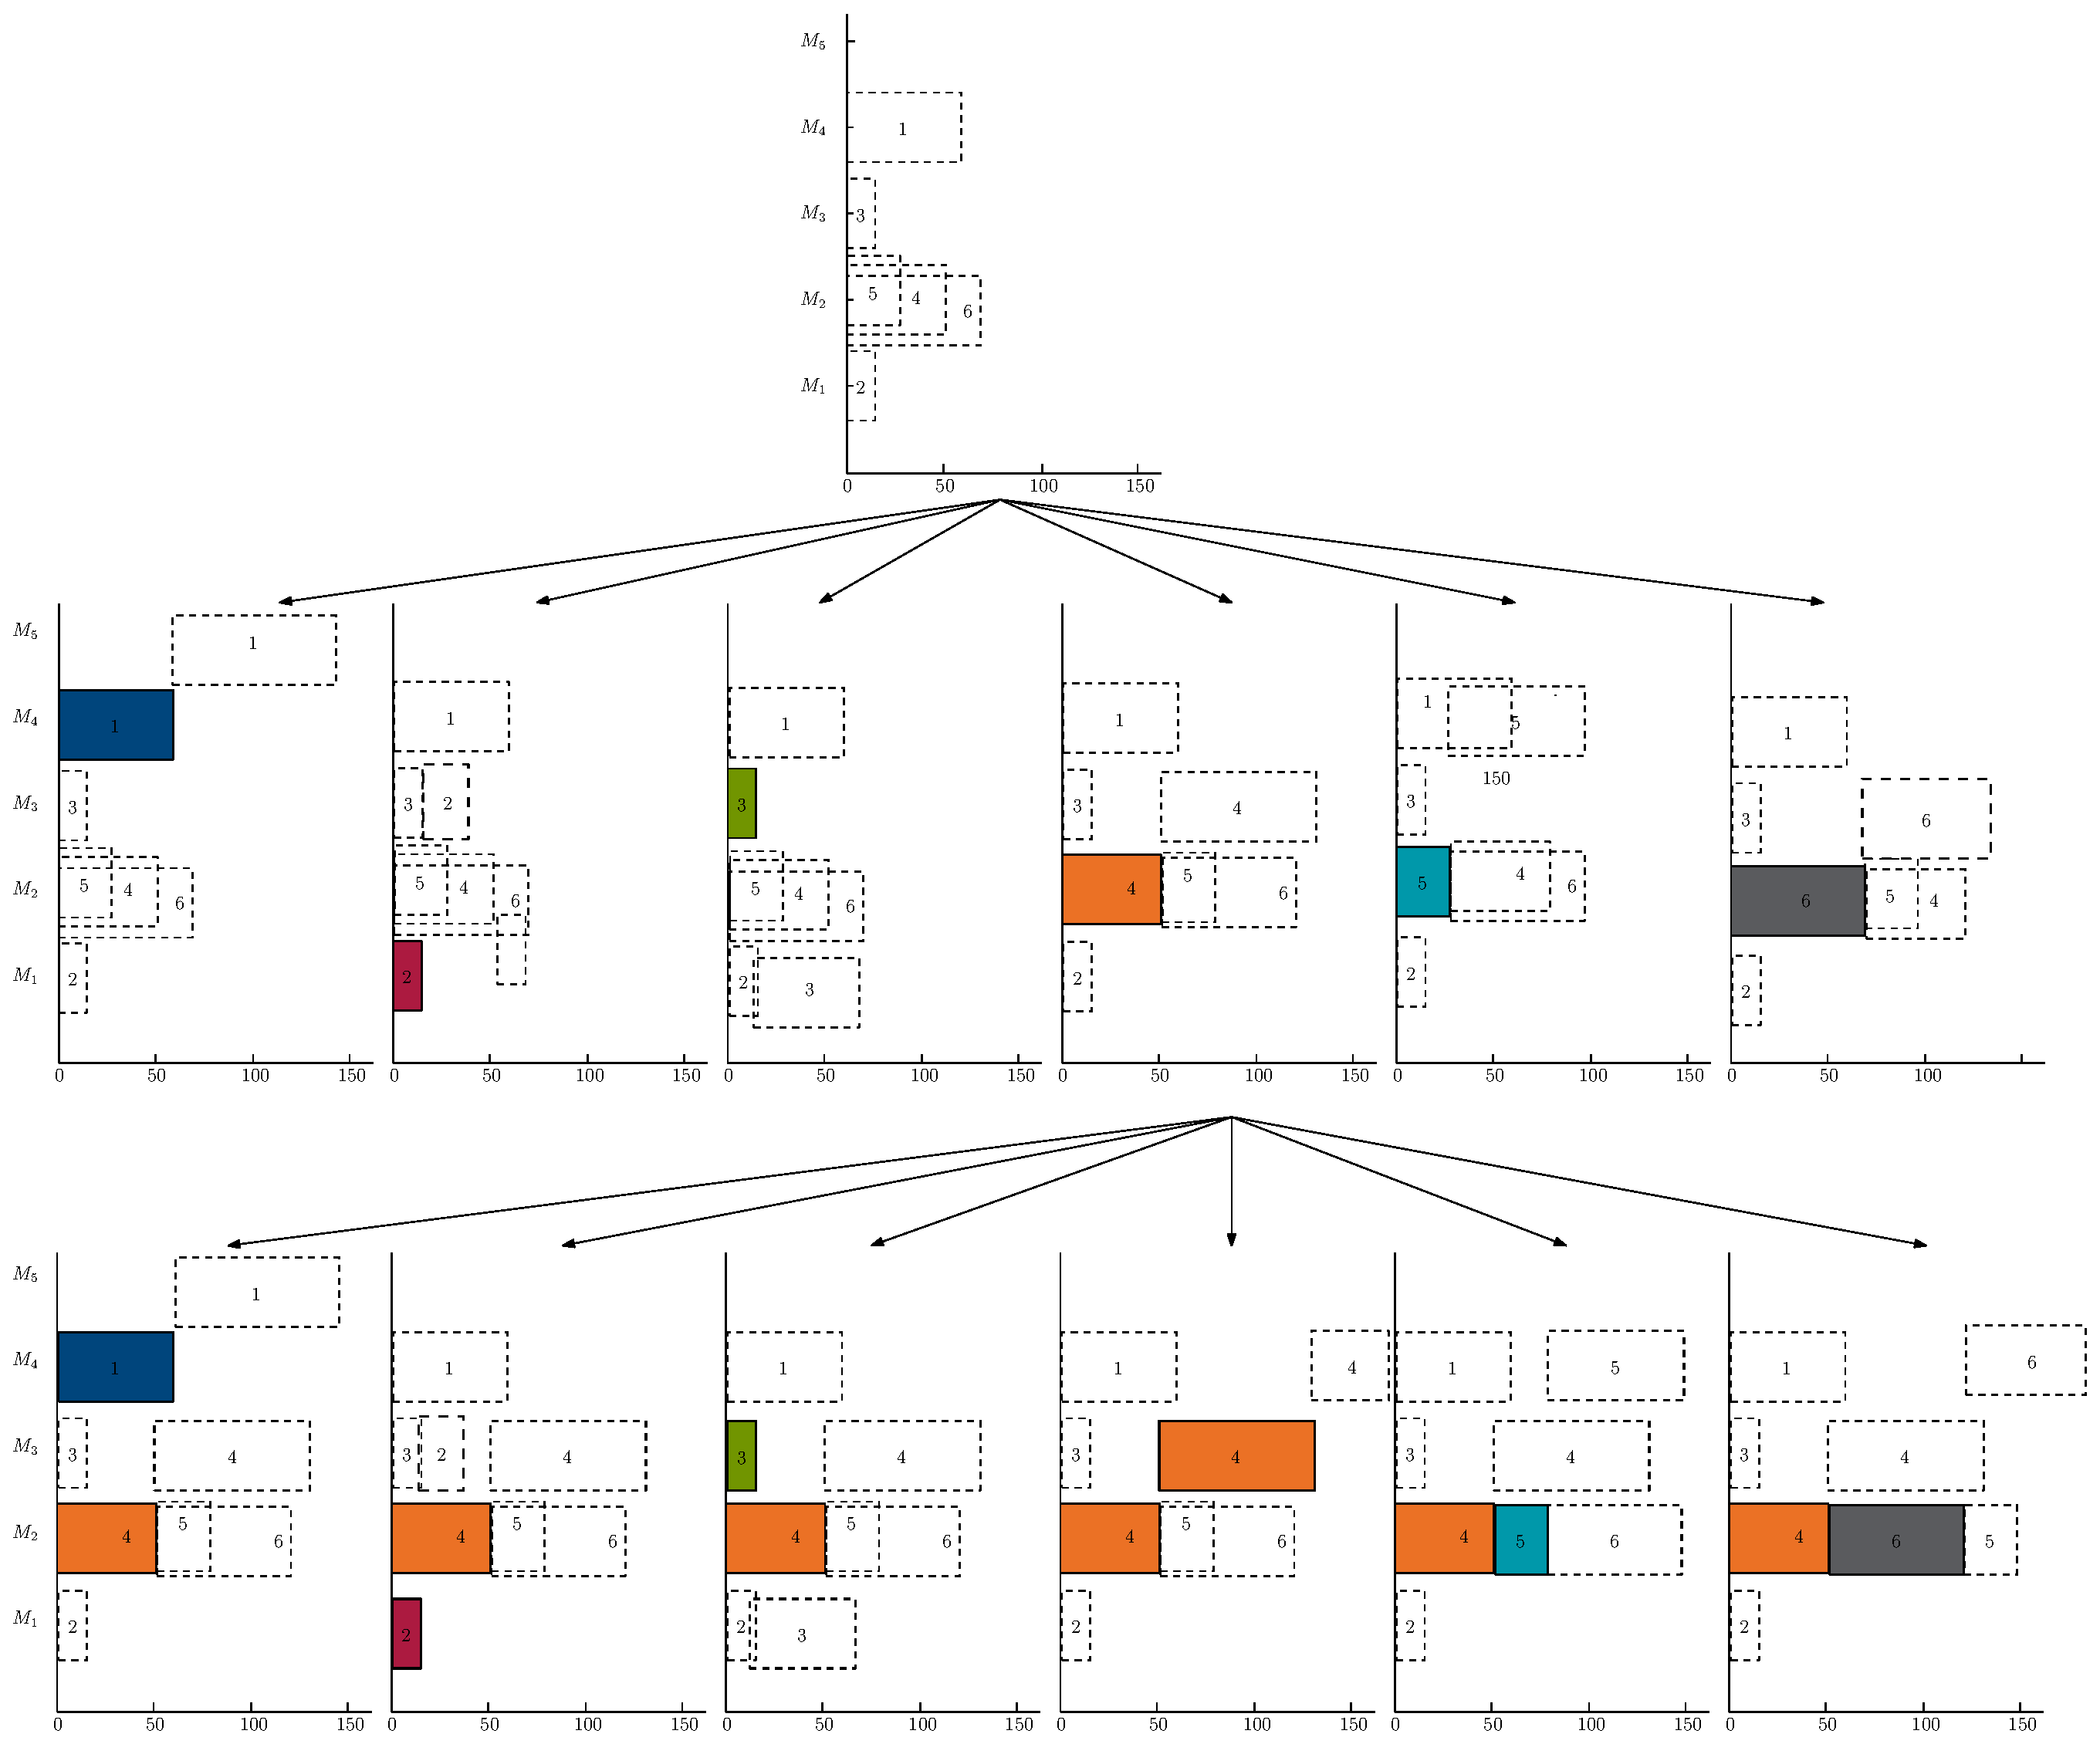
\includegraphics[width=\textwidth]{gametree}};
  \begin{scope}[x={(image.south east)},y={(image.north west)}]
  %% next four lines will help you to locate the point needed by forming a 
  %%grid. comment these four lines in the final picture.↓
  %\draw[help lines,xstep=.1,ystep=.1] (0,0) grid (1,1);
  %\draw[help lines,xstep=.05,ystep=.05] (0,0) grid (1,1);
  %\foreach \x in {0,1,...,9} { \node [anchor=north] at (\x/10,0) {0.\x}; }
  %\foreach \y in {0,1,...,9} { \node [anchor=east] at (0,\y/10) {0.\y};}
  %% upto here↑
  \node (J0) at (0.5,0.71) {};
  \node (J1) at (0.19,0.65) {};
  \node (J2) at (0.42,0.65) {};
  \node (J3) at (0.65,0.65) {};
  \node (J4) at (0.85,0.65) {};
  \draw[-latex] (J0) to[out=-20,in=+20] (J1);
  \draw[-latex] (J0) to[out=-20,in=+20] (J2);
  \draw[-latex] (J0) to[out=-20,in=+20] (J3);
  \draw[-latex] (J0) to[out=-20,in=+20] (J4);
  \node (J4) at (0.82,0.38) {};
  \node (J4J1) at (0.19,0.31) {};
  \node (J4J2) at (0.42,0.31) {};
  \node (J4J3) at (0.65,0.31) {};
  \node (J4J4) at (0.85,0.31) {};
  \draw[-latex] (J4) to[out=-20,in=+20] (J4J1);
  \draw[-latex] (J4) to[out=-20,in=+20] (J4J2);
  \draw[-latex] (J4) to[out=-20,in=+20] (J4J3);
  \draw[-latex] (J4) to[out=-20,in=+20] (J4J4);
  \end{scope}
  \end{tikzpicture}
}}
    \visible<3>{\resizebox{\columnwidth}{!}{\input{figures/example.graph.k10.tex}}}
    \\\vspace{24pt}
    \includegraphics<3>[width=\columnwidth]{figures/{example.gantt}.pdf}
    \end{column}
    \end{columns}
}
\frame{
    \frametitle{Mad Hatter tea-party (SDRs)}
    \includegraphics[width=\columnwidth,height=.9\textheight]{figures/{example.gantt.SDRs}.pdf}
}